
% This LaTeX was auto-generated from MATLAB code.
% To make changes, update the MATLAB code and republish this document.

\documentclass{article}
\usepackage{graphicx}
\usepackage{color}

\sloppy
\definecolor{lightgray}{gray}{0.5}
\setlength{\parindent}{0pt}

\begin{document}

    
    
\subsection*{Contents}

\begin{itemize}
\setlength{\itemsep}{-1ex}
   \item Extract raw data of sensor
   \item Plot w/ threshold value
\end{itemize}
\begin{verbatim}
clc; clear;

plotSpacing = 2;

% Create labels variable for subplots
labels = [ ...
" ",...
" ", ...
];

% Data source folder
dataFolder = 'FinalProject/';
% Pull all text files from source folder
fileNameList = ls('FinalProject/*.txt');
% Get number of files for looping and parsing
numOfFiles = size(fileNameList,1);


% Put all data in nested struct for organisation
%
for k = 1:numOfFiles

    % Prepend dataFolder for further parsing
    path(k) = string( ...
              strcat(dataFolder, fileNameList(k,:)) ...
              );

    % Read in data
    [dataSet(k).data, dataSet(k).t, dataSet(k).header] = ...
        BITalinoFileReader(path(k));

    % Assign labels for subplots from filenames
    labels(1,k) = fileNameList(k,:);

end
\end{verbatim}


\subsection*{Extract raw data of sensor}

\begin{verbatim}
figure(1)

for k = 1:numOfFiles
   rawData(k).acc = dataSet(k).data(:,6);

   % Plot rawData vs time in separate subplots
   subplot(numOfFiles,plotSpacing,k)
   plot(dataSet(k).t, rawData(k).acc)

   title(labels(1,k))
   xlabel('Time in sec'); ylabel('Raw Sensor');
   grid on;
   ax = gca;
   ax.XRuler.MinorTick = 'on';

end

sgtitle('Raw Data vs Time');
\end{verbatim}

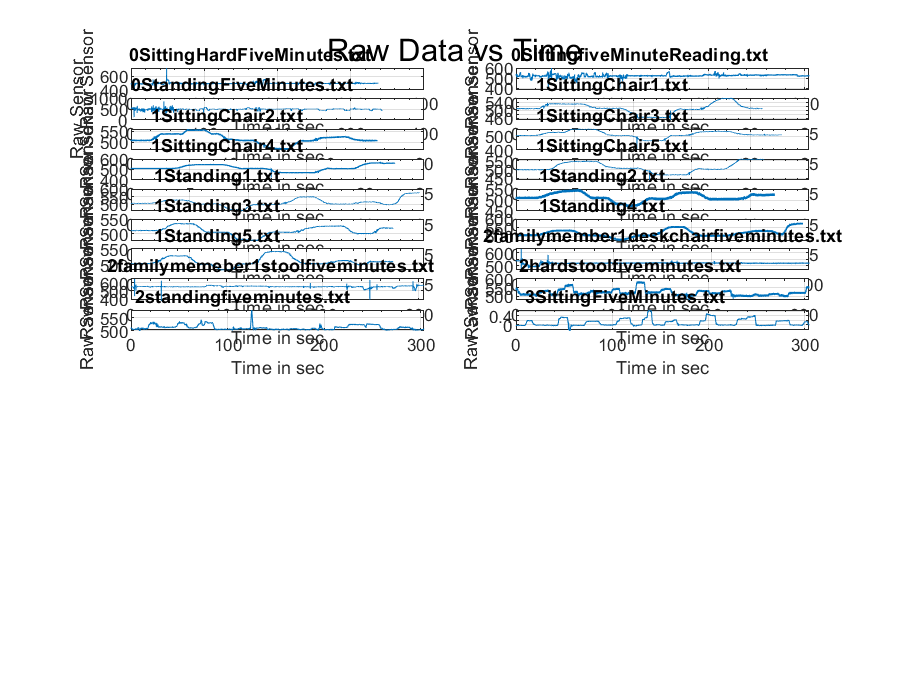
\includegraphics [width=4in]{FinalProject_01.eps}


\subsection*{Plot w/ threshold value}

\begin{verbatim}
ACCgThresh = 0.2;

for k = 1:numOfFiles - 1
   % These data points come from the LAB01/Data Calibration Recordings
   % files.
   CMin = 406;
   CMax = 618;

   % Equation comes from the ACC data sheet using best fit from rotating
   %    along the Z-axis per the data sheet

   %  ACCg = 2 * (rawData(k).acc - min(rawData(bestCalFit).acc) ) / ...
   %  (max(rawData(bestCalFit).acc) - min(rawData(bestCalFit).acc) ) - 1;

   % Using Cmin and CMax from leaving the ACC on desk.
   ACCg = ( (rawData(k).acc - CMin ) / (CMax - CMin) ) * 2 - 1;

    Fs = dataSet(k).header.samplingrate;   % Sampling frequency
    T = 1/Fs;                                      % Sampling period
    L = length(dataSet(k).data);           % Length of signal
    f = Fs*(0:(L/2))/L;

% plot each on own figure for ease of use in report
%   figure(k)
%    plot(dataSet(k).t,ACCg)

    x = dataSet(k).t;
    y = ACCg;

% Using a cutoff of: -ACCgThresh <= y >= ACCgThresh
    Cutoff = y;
    Cutoff(y >= -ACCgThresh & y <= ACCgThresh) = NaN;  % Replace points above cutoff with NaNs;

    figure;
    plot(x,y,'b',x, Cutoff, 'r');

   title(labels(1,k))
   yline(ACCgThresh,'--r')
   yline(-ACCgThresh,'--r')
   xlabel('Time in sec'); ylabel('g, (9.8 m/s^2)');
   legend("ACC g normalised, ", "\pm " + ACCgThresh + " g threshold");

   grid on;
   ax = gca;
   ax.XRuler.MinorTick = 'on';

   %
   Cutoff = y;
   Cutoff(y >= -ACCgThresh & y <= ACCgThresh) = 0;

   [R, C]=find(Cutoff);

end


% Plot converted data by itself for ease of plotting.

    k = numOfFiles;
    x = dataSet(k).t;
    y = rawData(k).acc;

% Using a cutoff of: -ACCgThresh <= y >= ACCgThresh
    Cutoff = y;
    Cutoff(y >= -ACCgThresh & y <= ACCgThresh) = NaN;  % Replace points above cutoff with NaNs;

    figure;
    plot(x,y,'b',x, Cutoff, 'r');

   title(labels(1,k))
   yline(ACCgThresh,'--r')
   yline(-ACCgThresh,'--r')
   xlabel('Time in sec'); ylabel('g, (9.8 m/s^2)');
   legend("ACC g normalised, ", "\pm " + ACCgThresh + " g threshold");

   grid on;
   ax = gca;
   ax.XRuler.MinorTick = 'on';

   %
   Cutoff = y;
   Cutoff(y >= -ACCgThresh & y <= ACCgThresh) = 0;

   [R, C]=find(Cutoff);
\end{verbatim}

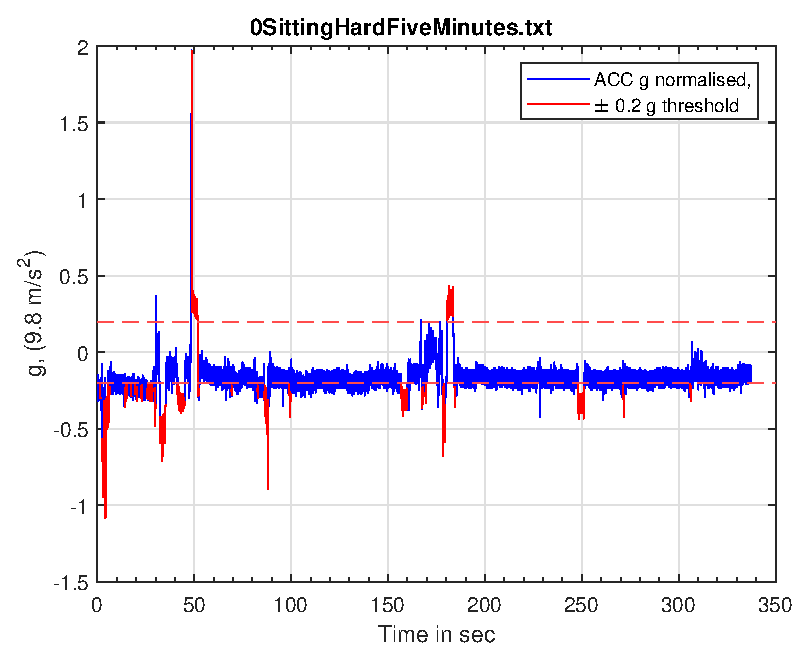
\includegraphics [width=4in]{FinalProject_02.eps}

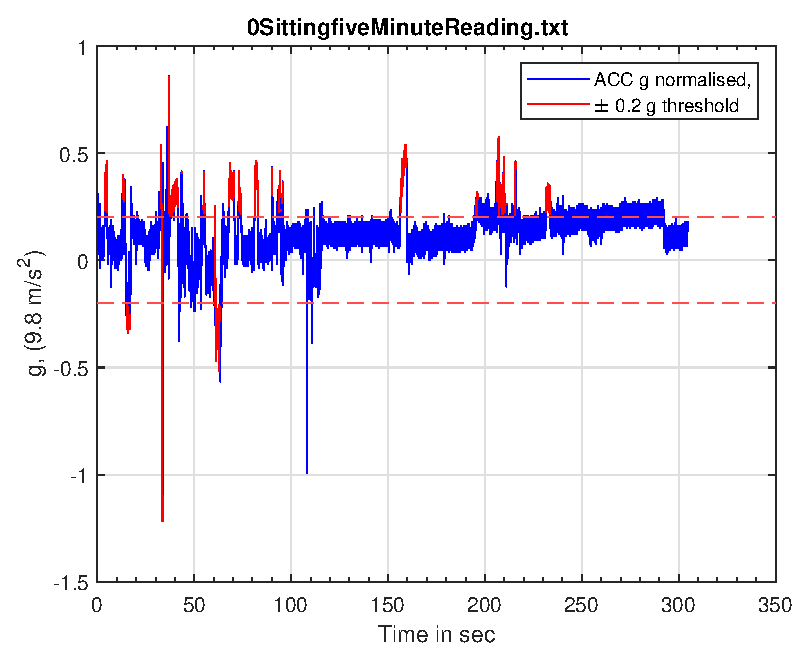
\includegraphics [width=4in]{FinalProject_03.eps}

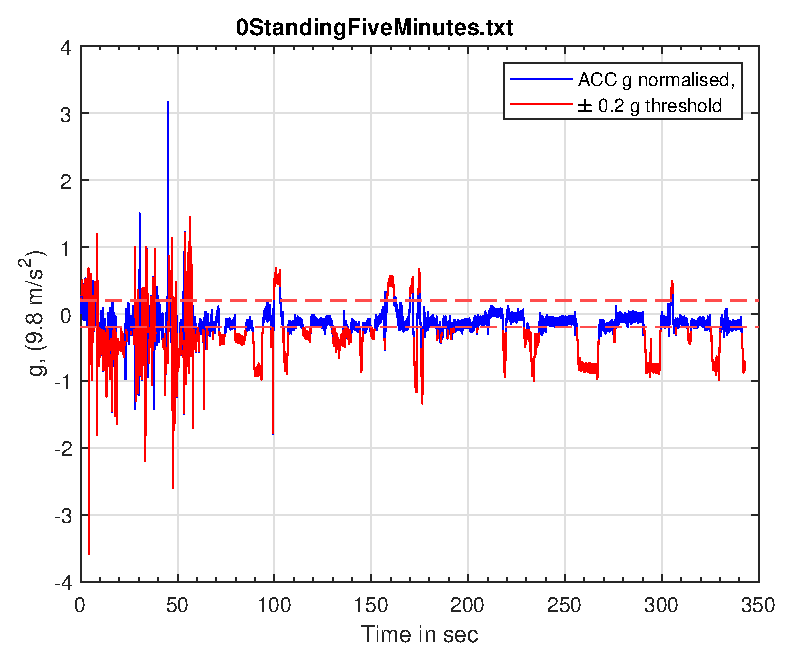
\includegraphics [width=4in]{FinalProject_04.eps}

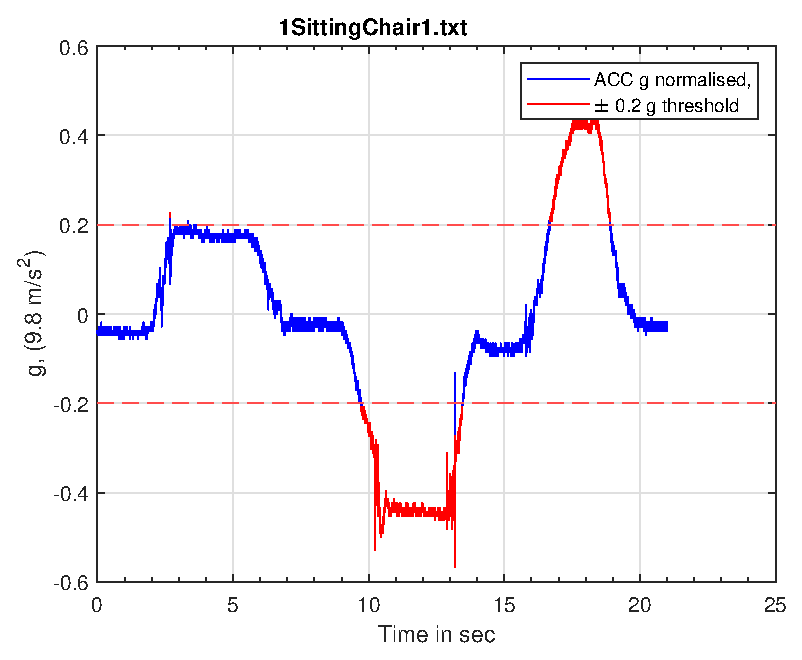
\includegraphics [width=4in]{FinalProject_05.eps}

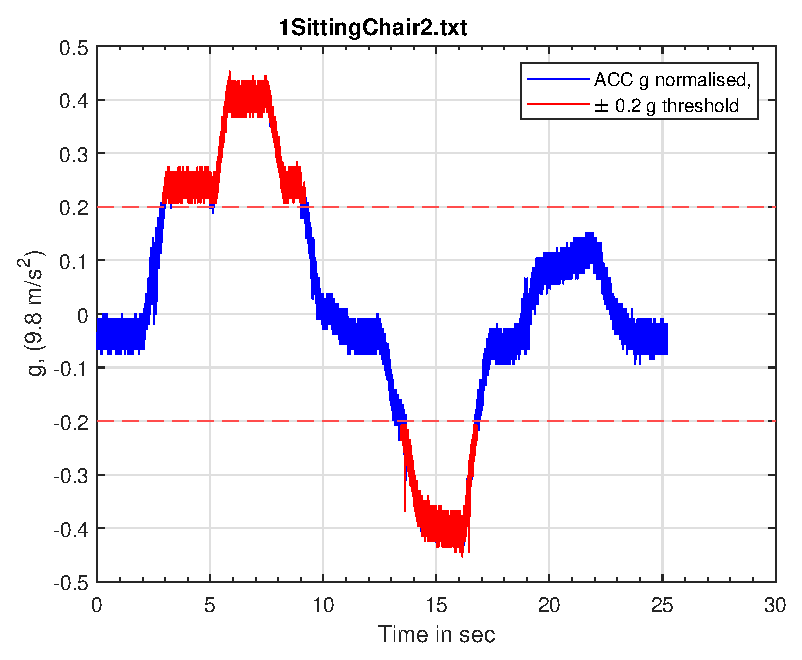
\includegraphics [width=4in]{FinalProject_06.eps}

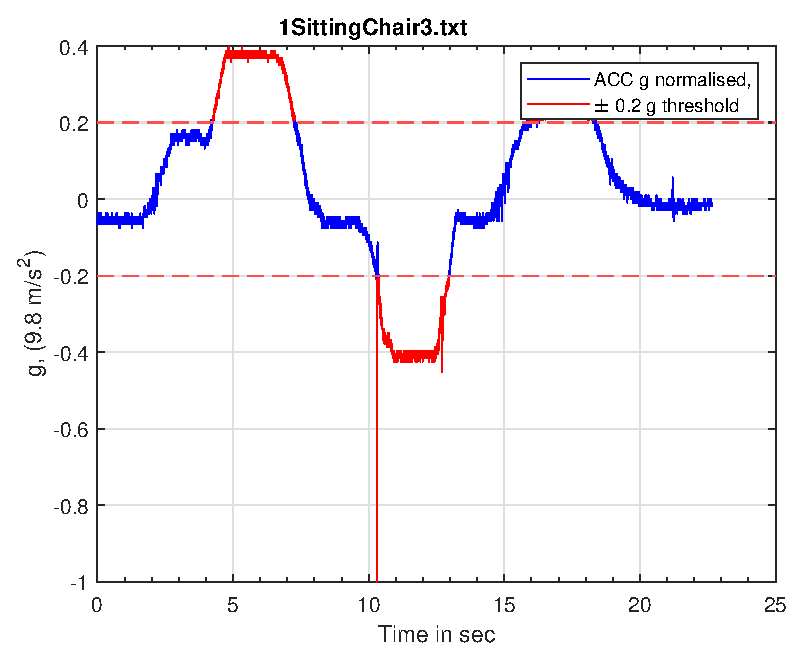
\includegraphics [width=4in]{FinalProject_07.eps}

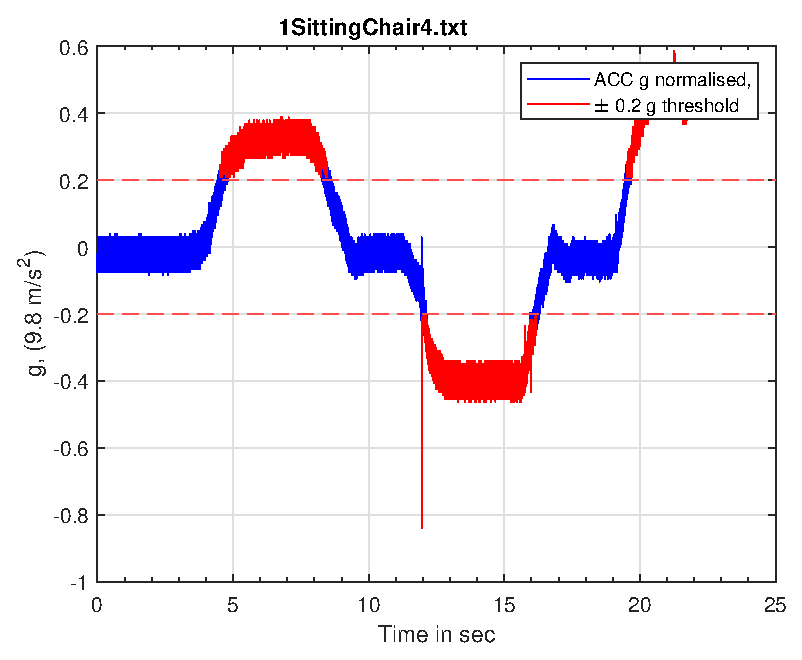
\includegraphics [width=4in]{FinalProject_08.eps}

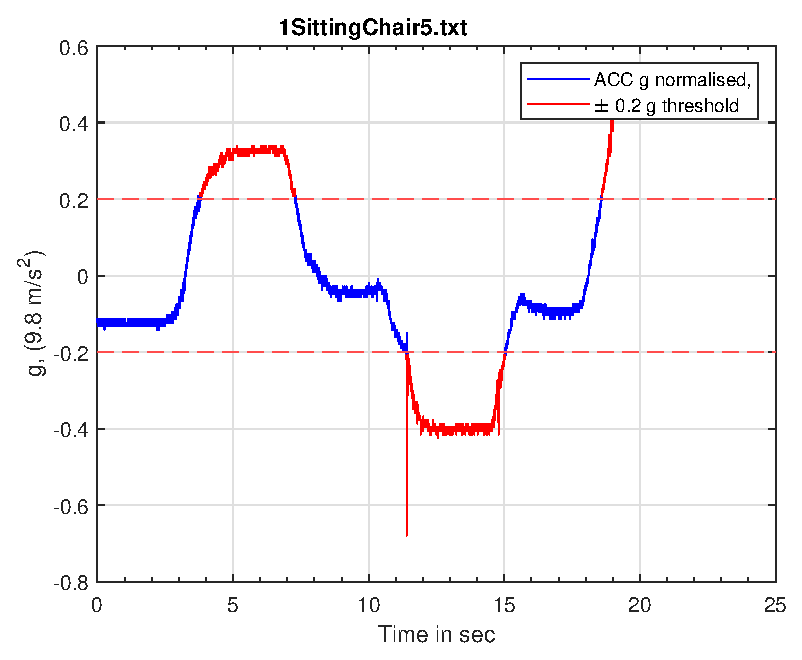
\includegraphics [width=4in]{FinalProject_09.eps}

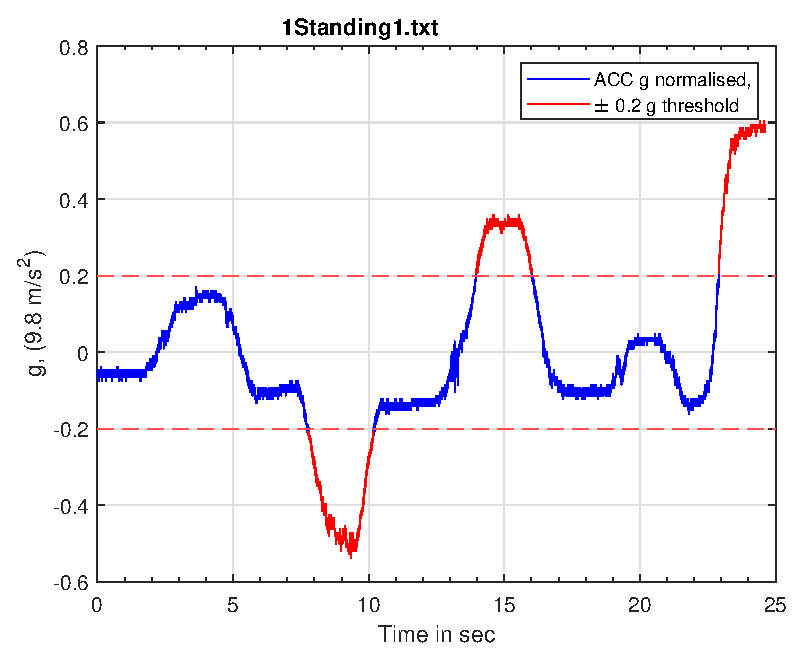
\includegraphics [width=4in]{FinalProject_10.eps}

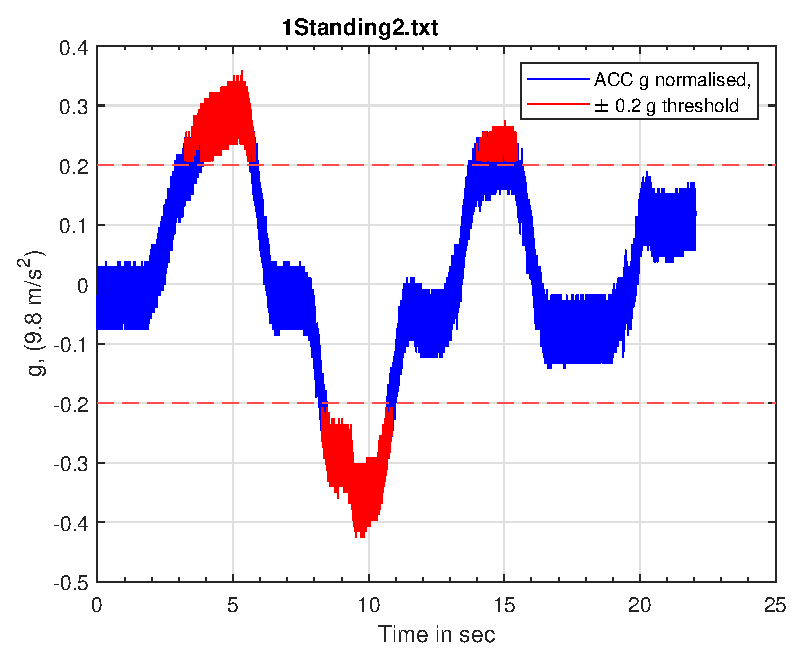
\includegraphics [width=4in]{FinalProject_11.eps}

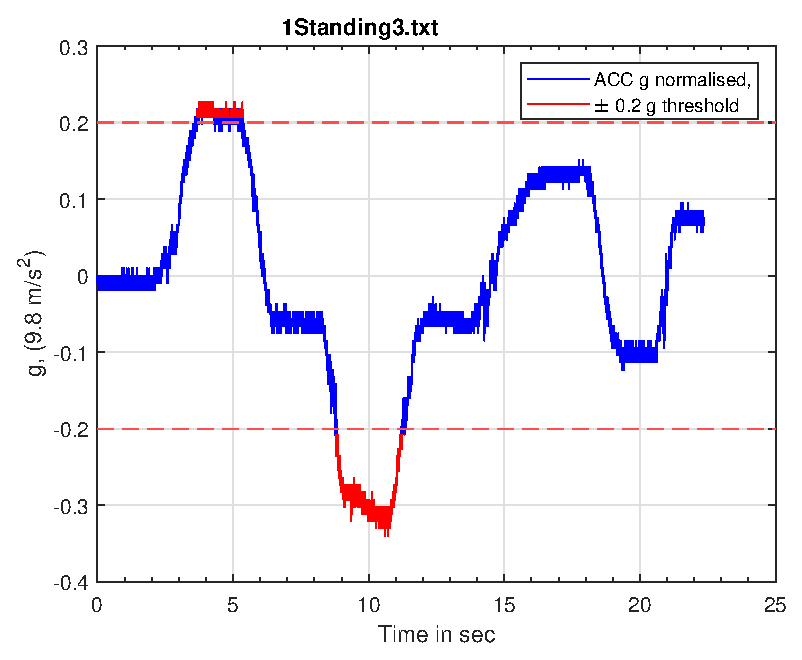
\includegraphics [width=4in]{FinalProject_12.eps}

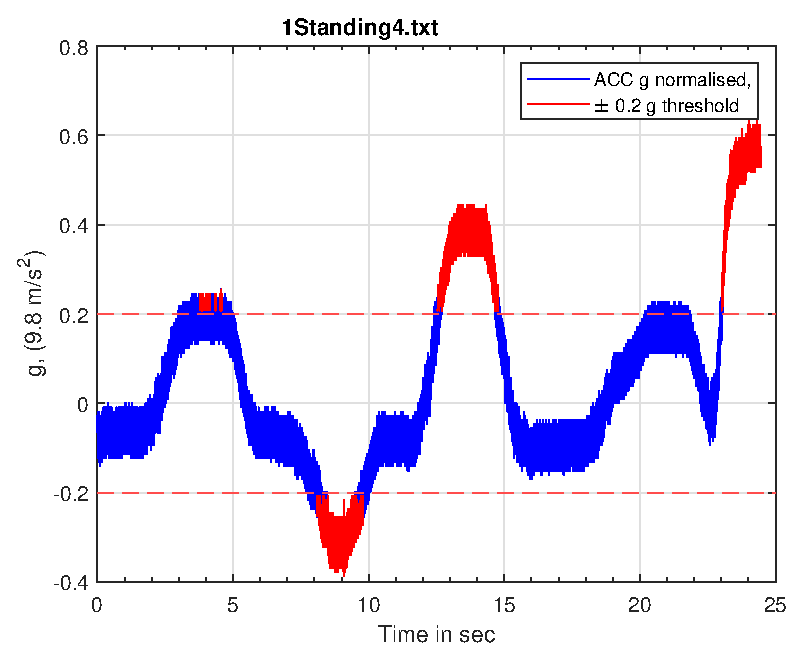
\includegraphics [width=4in]{FinalProject_13.eps}

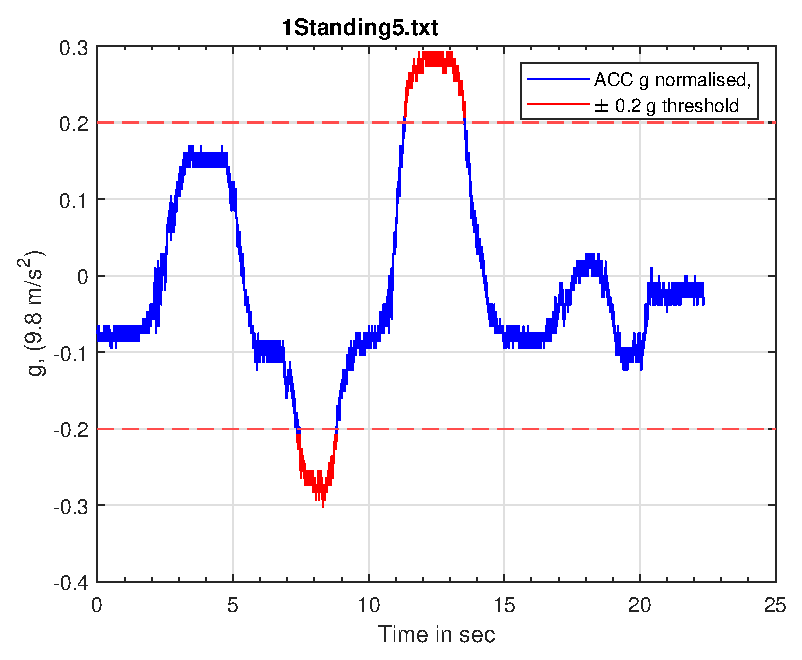
\includegraphics [width=4in]{FinalProject_14.eps}

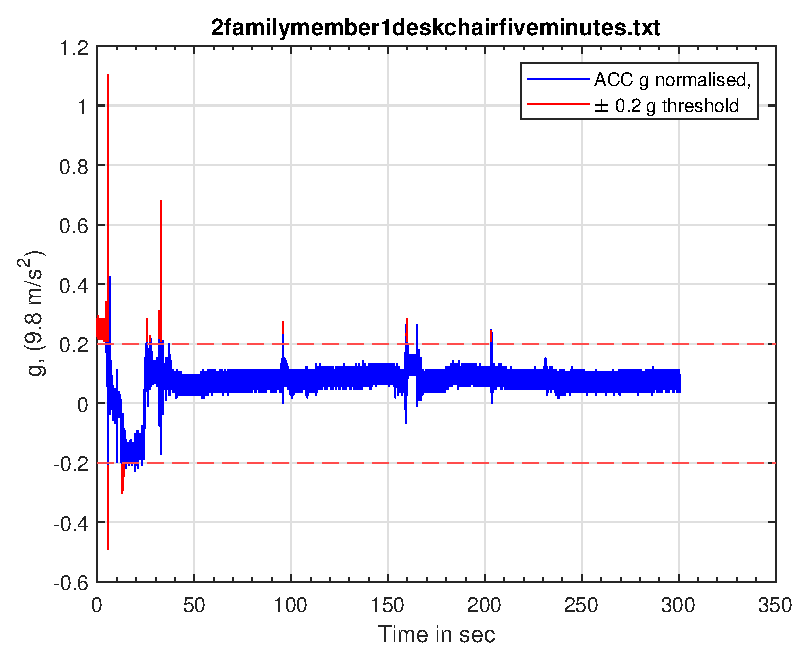
\includegraphics [width=4in]{FinalProject_15.eps}

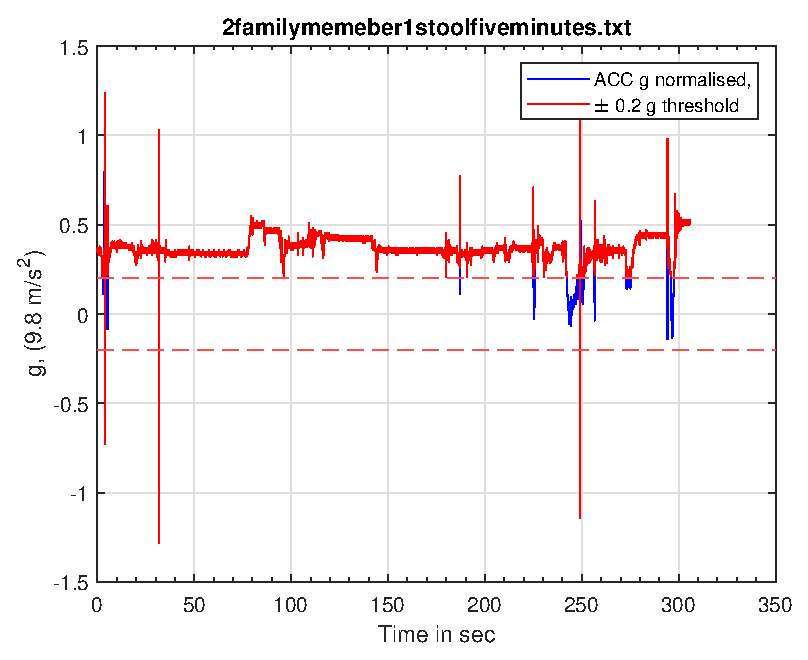
\includegraphics [width=4in]{FinalProject_16.eps}

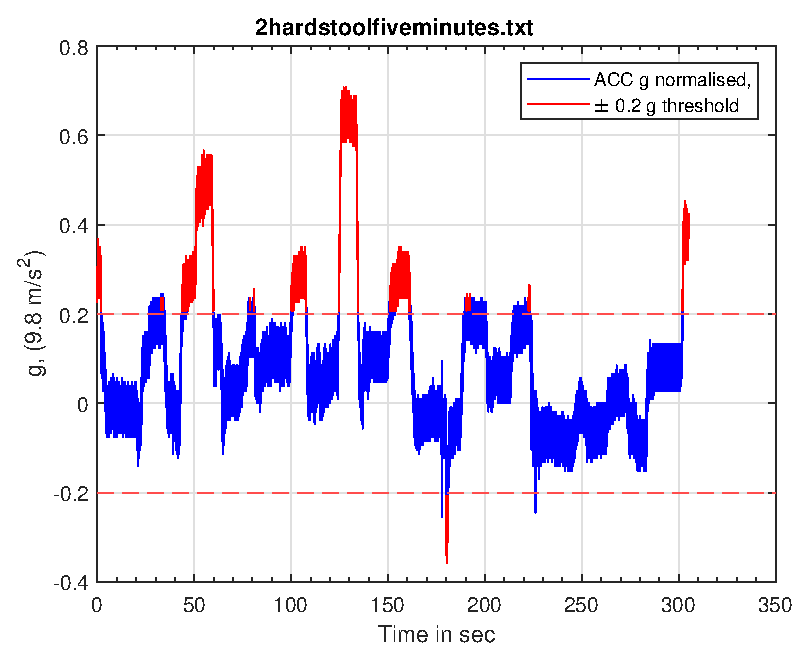
\includegraphics [width=4in]{FinalProject_17.eps}

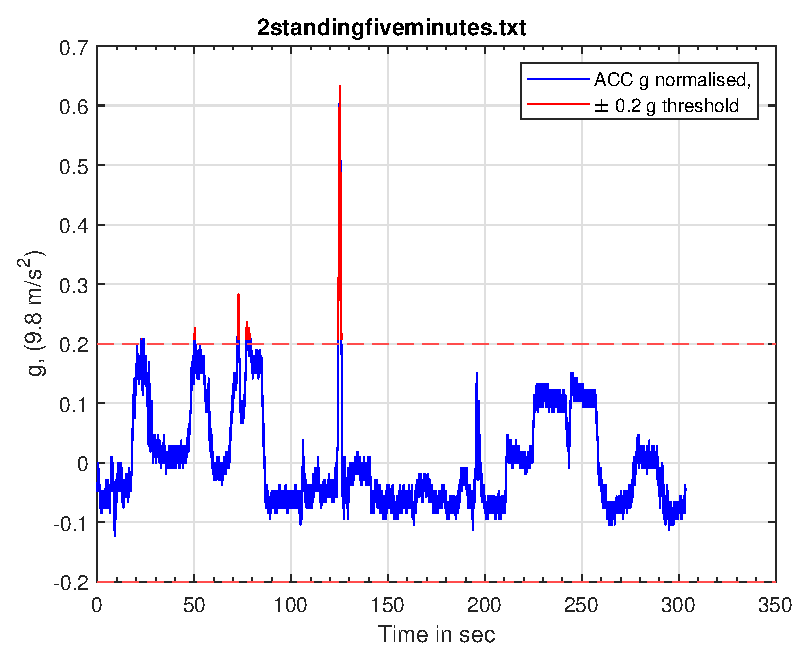
\includegraphics [width=4in]{FinalProject_18.eps}

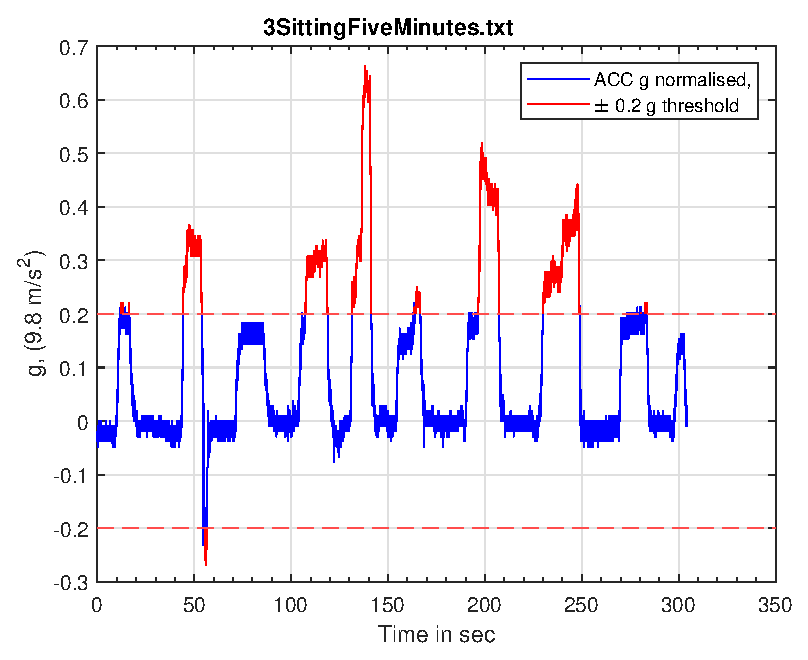
\includegraphics [width=4in]{FinalProject_19.eps}



\end{document}

